This chapter contains the description of the development and our experiences
from the project.

\section{Team}

The team consists of five members. Petr has been elected as team leader,
mostly because of his reliability and hard-working nature. The work has been
divided according to members' interests and knowledge after fruitful discussion.


\paragraph{Bc. Petr Fanta}
\begin{itemize}
\item team leader
\item responsible for server components interconnection especially layered
design, server configuration, communication design
\item implemented webservice layer, service layer, scheduler, full text search and testing
\end{itemize}
\paragraph{Duc Tam Hoang, B. Sc.}
\begin{itemize}
\item responsible for entity-object assignment
\item implementation of entity-object assigner and tests, documentation
proof-reading
\end{itemize}
\paragraph{Bc. Adam Huječek}
\begin{itemize}
\item responsible for client
\item implemented client application, command line interfaces, documentation
proof-reading, code review
\end{itemize}
\paragraph{Bc. Václav Pernička}
\begin{itemize}
\item responsible for database and persistence layer
\item implemented database schema, graph operations, DAOs, ORM
\end{itemize}
\paragraph{Bc. Jakub Vlček}
\begin{itemize}
\item responsible for NameTag and MorphoDiTa integration
\item implemented the integration, training data preparation
\end{itemize}

\section{Work on the Project}

%This section contains work progress
%In this section is described work progress in each iteration.
This section provides details of the work progress in each iteration, decisions
we made and issues we solved.

\subsection{Beginnings}
\textan{} team visited policeman plk. Ing. Jan Hořínek, who introduced us to his
work and showed us the existing inadequate software. We were asked to prepare
a tool that would help the Police with processing such large amounts of
documents. Basis of the project was processing police reports - recognize
entities and match them to existing objects in the database. We were advised to
use Webservices for an easy integration of the project to the current system. He
promised us models and example data inputs. The problem is quite universal, so
we have decided to provide a general solution that could be deployed in many
domains with as least additional work.

We made some decisions and requirements for each component:

\paragraph{Database}
At the beginning, we made the database schema (see Figure\ref{fig:dbpilot}),
which was improved over a few iterations. The main attention was paid on schema
generality because we want to support more than one domain (not just police
report). Database should support versioning, parallel processing and partial
records. We decided to create a special layer between server and database
because of generality (it is be easier to change the database system). Logging
(users, changes) support is also required. It would be a problem merging two
objects into  one, so we created special functionality and table in the
database.

\begin{figure}[!htb]
        \centering
        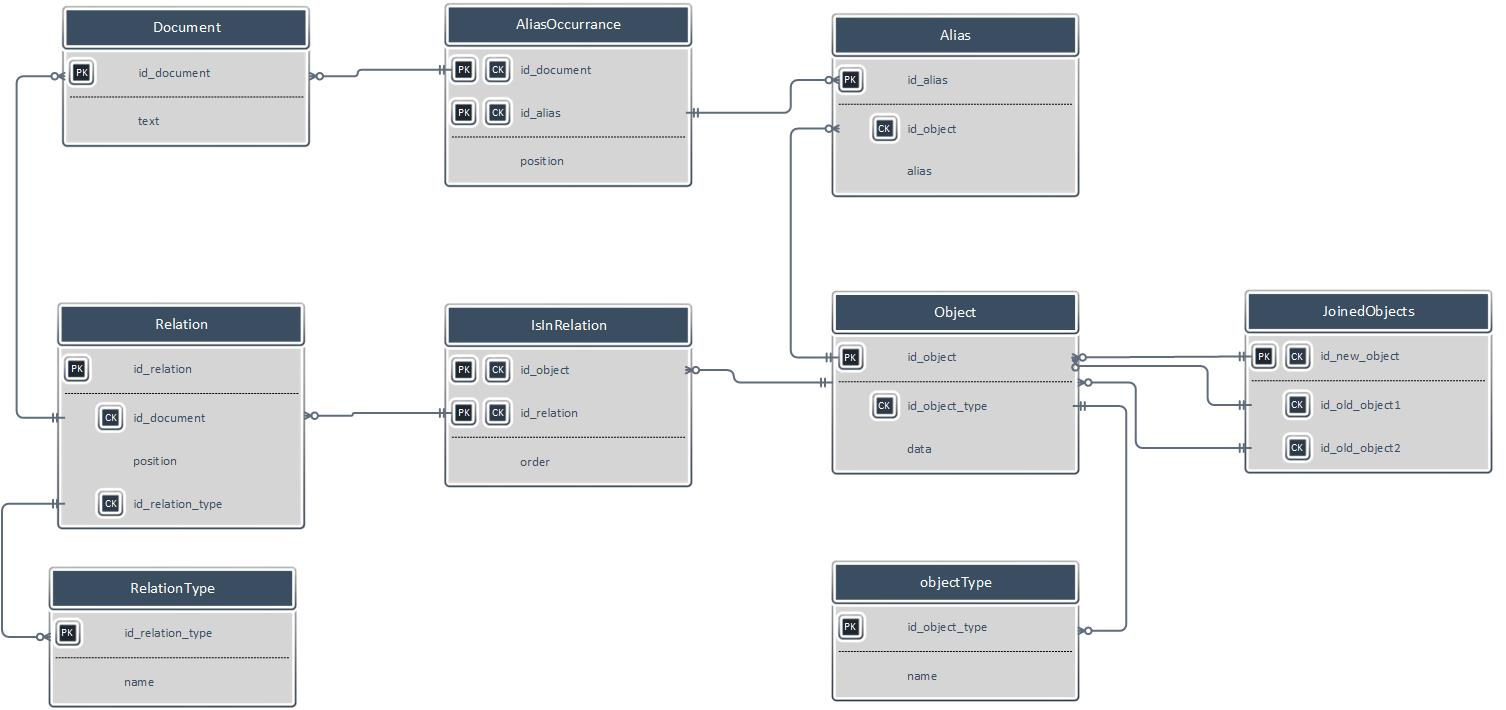
\includegraphics[width=\textwidth]{Images/db-pilot}
        \caption{Pilot database schema.}
        \label{fig:dbpilot}
\end{figure}

\paragraph{Client}
We decided to use pipeline model. In other words, the report processing consists
of several phrases:

\begin{enumerate}
\item Report insertion
\item Report editing
\item (Auto) Entity recognition
\item Entity editing (entity types, ranges, creating new ones)
\item (Auto) Object recognition
\item Object editing (adding new ones, repair bad connections between entities and objects)
\item (Auto) Relationships recognition
\item Relationships editing
\item Report confirmed and sent to server
\end{enumerate}

Changes in each phase are not stored in the database immediately but stored
locally. They would be stored to the database at the end of the pipeline. There
was problem with machine recognition, because models with newly added items are
trained after final confirmation, so it is impractical to learn from the
incomplete user input. We decided that newly added items will be displayed next
to automatically assigned ones so users can correct the server outputs easily.
 
\subsection{Design \& Technologies}
In the next period, we mainly chose and tested technologies which we could use.
New member Duc Tam Hoang joined \textan{}. His specialization is linguistic and
machine learning so he is be really useful for our project. Because of Tam's
limitation in Czech, the documentation language was changed to English. His main
task will be NER and entity-object matching. We were trying different
entity recognizers, but there are not many applicable for Czech. Milan Straka
promised us his project \emph{NameTag}. It is named entity recognizer for Czech,
so exactly what we need. Problem is that it is not finished yet and it is coded
in C++ language, so there must be additional layer between Java and C++.
We researched possibilities about entity-object matching. Program would get
entity and assign it possible candidates from objects stored in the database.
This part could not be purely automatic because of ambiguity, but if there will
be high probability, program should match object entity pair automatically.

Possible solutions for entity-object matching are machine learning methods
ranking or classification.

We looked for suitable Java library which provides machine learning techniques.
Candidates were JavaML and Weka. We have tested them both and at first, we chose
JavaML, because it provides more machine learning algorithms (some of them uses
WEKA library) and because of WEKA problem - it has been created for teaching
purposes so its performance is not as good as JavaML. Then we found that we
do not need these functions and because JavaML seems no longer be supported and
that new version of WEKA was released, we choose WEKA, because it is a live
project and its functionality is good enough for our needs.

There were two possible server architectures: standalone or embedded webserver
(Tomcat or Jetty). We have decided to use embedded sever because it is easier to
deploy. We considered usage of some technologies like Spring, CXF and
Hibernate for database layer.

\subsection{Prototyping \& Interconnecting}
After the technologies were chosen, we made some prototypes of each component.
We discussed a lot of APIs (we need them for testing). For testing purposes, we
had to provide some mock objects, so everyone implemented a mock of his
component. \emph{NameTag} was beta-released, so we tried to get acquaintance. We
met Milan Straka, the author of \emph{NameTag}. He presented his library and
helped us get familiar with it. We started testing it. There were problems with
compiling (it did not support Windows from the beginning) and Java bindings
whose solving took more time than we expected. Problem was mainly missing
documentation as the project was still in development too. We connected the
client and the database to server, implemented database data browsing on client
(mainly graphs viewing with JUNG). Tam made prototype of object matcher, but it
was not integrated to server.

\subsection{Main Coding}
When we made a prototype of the whole syste, everyone started improving his
component in his own branch.

\paragraph{Server} Server was debugged and made reliable. The original idea of
generating WSDL from Java code was scraped. It started using hand-made WSDLs 
so there were lot of work on both server and client parts. Result was that Java
code is now generated automatically from the WSDLs and not vice-versa.
Connection to the database was reworked to use Spring Beans.

\paragraph{Named entity recognizer} NameTag was fully integrated to server. We 
started adapting it for our purposes (using our structures and types). There
were problems with gazetteers files and translating entities from NameTag to
\textan{}. After receiving information that NameTag will not support JNI to
training parts we researching how to launch training binaries from Java which
is more complicated as both 32 and 64 bit operating systems should be supported.

\paragraph{Client} Client implemented the pipeline, we improved graph viewing to
support oriented edges.

\paragraph{Object matcher} TextPro (as we called entity-object matching in that
time) has first prototype. It uses a simple ranking method, which resulted in a
poor performance. 

\paragraph{Database} Database has a new layer with DAOs, so no more need to
access database directly. After this iteration, we released first alpha version
of TextAn.

\subsection{Improving}
The alpha version of NameTag learning was implemented. There were few problems
with portability because of different architectures and operating systems. After
implementing special functions in database, we made automatic data extraction
for learning. For this purpose, new function to server was added - commands. It
is the implementation of design pattern Command which starts data generation and
model training after new report insertion. Models managing implemented due to
bigger size (and deleting old ones). Database support logging. It was done
through interceptors - triggers in Hibernate layer. In the client, there were
lots of small fixes in GUI, problems were with portability between Windows and
Unix-like systems, where ControlsFX and JavaFX behave differently. TextPro
received many new features. We integrated Morphodita because we needed its
tagger for new features. Settings through properties files are now supported in
each component.

\subsection{Bugfixing \& Testing}
The most important parts of the code are covered by unit tests. Webservices have
been tested by SoapUI. The project was tested on real dat. For final testing, we
have created a server hosted by Charles university with address
\url{textan.ms.mff.cuni.cz:9500}. Here we always keep the newest version from
the master branch.

\section{Lessons Learned}
\comment[all]{Adam}{Add your experience with the project}
\comment{Adam}{Maybe scrap the whole section?}

\paragraph{Tam}
I was introduced to the project by surprise. However, working on \textan{} project
with other members help me learn useful things. Firstly, it is an opportunity to look at
machine learning from the view of industry. It is not only the practical session to transform a
real problem into a classification problem but also a chance to implement the solution in
a software. Secondly, I gain knowledge in software project, especially in writing documentation.
With regards to my main role in the project (entity\-object assigner), it is a requirement to
implement a machine learning in JAVA, specially JavaML. 
I did not have a pleasure experience working with JavaML. However, I played with it long enough to
understand the strong points and weak points. Finally, we decided to changed to Weka instead of keeping
JavaML.
 
\comment{Adam}{mention standartized logging.}